\documentclass[12pt]{article}

\usepackage[utf8]{inputenc}
\usepackage{sfmath}
\usepackage{amsmath}
\usepackage{graphics}
\usepackage{graphicx}
\usepackage{subfig}
\usepackage{wrapfig}
\usepackage{lipsum}

\usepackage[super, sort&compress]{natbib}
\usepackage{hyperref}
\usepackage{url}

\usepackage{tikz}
\usetikzlibrary{shapes.geometric}
 
\usepackage{physics}

\usepackage{titling}
\pretitle{\begin{center}\Huge\bfseries}
\posttitle{\par\end{center}\vspace{0.5cm}}
\preauthor{\begin{center}\large}
\postauthor{\par\end{center}}
\predate{\begin{center}\large}
\postdate{\par\end{center}}

\usepackage{geometry}
\geometry{a4paper, margin=1in}

\title{
    Mechatronics and Making \\
    Mid-Term Project Report \\
    Exoskeleton Robotic Hand With Wolf Claw Mechanism
}


\author{
    \begin{align*}
        \text{Bryan Li}\ &-  \text{SN 25003743} \\
        \text{Yan Pei Zhu}\ &-  \text{SN 25103352}\\
        \text{Nolan Yu}\ &-  \text{SN 25113715}
    \end{align*}
}

\date{October 31, 2025}

\setlength{\parindent}{0pt}
\setlength{\parskip}{1em}


\begin{document}

\begin{titlepage}
	\maketitle
\end{titlepage}

\tableofcontents

\pagebreak

% ======== SECTION I ==========

\section{Introduction}
\subsection{Project Objectives and Description}
\subsection{Similar Mechanisms}
\subsection{Industrial Applications}

\pagebreak

% ======== SECTION II =========

\section{Mechanical and Mechanism Analysis}

\subsection{Drive Method and Transmission}
This robotic hand exoskeleton uses an acceleration-based machinery system, 
amplifying the movements of the finger. 

This is achieved using a planetary gear mechanism connected to a string 
transmission and a pulley and belt system.

Details of the transmission process shown below:

\begin{center}
	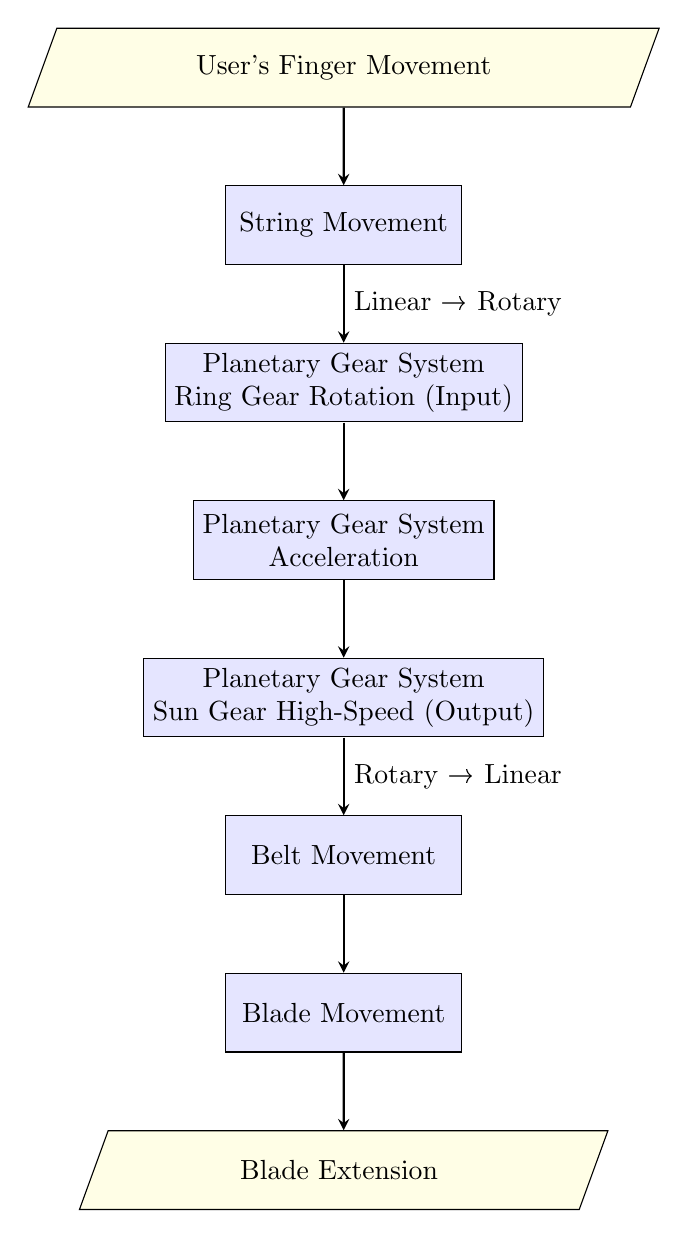
\begin{tikzpicture}[scale=0.8]

		% Define styles
		\tikzstyle{process} = [
		rectangle, minimum width=3cm, minimum height=1cm,
		text centered, draw=black, fill=blue!10, align=center]
		\tikzstyle{io} = [
		trapezium, trapezium left angle=70,
		trapezium right angle=110, minimum width=3cm,
		minimum height=1cm, text centered, draw=black,
		fill=yellow!10, align=center]
		\tikzstyle{arrow} = [thick,->,>=stealth]

		% Nodes
		\node (start) [io] {User's Finger Movement};

		\node (tendon) [process, below of=start, yshift=-1cm] {String Movement};

		\node (ring) [process, below of=tendon, yshift=-1cm] {
			Planetary Gear System \\
			Ring Gear Rotation (Input)
		};

		\node (planetary) [process, below of=ring, yshift=-1cm] {
			Planetary Gear System \\
			Acceleration
		};

		\node (sun) [process, below of=planetary, yshift=-1cm] {
			Planetary Gear System \\
			Sun Gear High-Speed (Output)
		};

		\node (pulley) [process, below of=sun, yshift=-1cm] {Belt Movement};

		\node (belt) [process, below of=pulley, yshift=-1cm] {Blade Movement};

		\node (blade) [io, below of=belt, yshift=-1cm] {
			Blade Extension
		};


		% Arrows
		\draw [arrow] (start) -- (tendon);
		\draw [arrow] (tendon) -- node[right] {Linear → Rotary} (ring);
		\draw [arrow] (ring) -- (planetary);
		\draw [arrow] (planetary) -- (sun);
		\draw [arrow] (sun) -- node[right] {Rotary → Linear}(pulley);
		\draw [arrow] (pulley) -- (belt);
		\draw [arrow] (belt) -- (blade);
	\end{tikzpicture}
\end{center}

\pagebreak

\subsection{Hand Exoskeleton Mechanisms}

\subsubsection{Hand Biomechanics}
Most human hands have 19 bones and 14 joints\cite{heo2012current}, excluding the carpal bones.

The design of the hand exoskeleton needs to be based on the natural anatomy of the 
human hand~(figure~\ref{fig:hand_skeleton}). We have to focus on MCP, PIP, and 
DIP joints, because they ensure the finger can flex and extend easily.

\begin{figure}[htbp]
	\centering
	\includegraphics[width=0.4\textwidth]{imgs/bones_joints_of_hand.png}
	\caption{bones and joints of a human hand\cite{heo2012current}}\label{fig:hand_skeleton}
\end{figure}

The finger joints include 3 types of joints majorly\cite{rosen2019wearableC8}:

Metacarpophalangeal Joint (MCP): \\
Has 2 degrees of freedom (flexion/extension, abduction/adduction).

Proximal Interphalangeal Joint (PIP): \\
Has 1 degree of freedom (flexion/extension).

Distal Interphalangeal Joint (DIP): \\
Has 1 degree of freedom (flexion/extension).

In the resting posture, the angle of MCP joint is approximately 45°, 
whereas the PIP joint is between 30°--45°, and the DIP joint is between 10°--20°. 
To define the range of motion and ensure safety in exoskeleton design, 
it is essential to align our mechanism to the human anatomy. 

\textbf{Wrist Structure Analysis}

The wrist has 2 degrees of freedom: flexion/extension and radial/ulnar deviation. 

\subsubsection{Selection of Mechanism Type}


Among the mechanisms illustrated in 
Figure~\ref{fig:mechanism_types}, the direct matching of joint 
centers (Figure~\ref{fig:mechanism_types}.a) was 
selected for our design because it provides a  
simple and compact solution without requiring additional 
linkages or complex actuation. 
Also, this approach minimises the mechanical complexity, 
reduces system weight, and simplifies both fabrication and control.

\begin{figure}[htbp]
    \centering
    \includegraphics[width=0.88\textwidth]{imgs/mechanism_types.png}
    \caption{mechanism types\cite{heo2012current}\cite{rosen2019wearableC8}}\label{fig:mechanism_types}
\end{figure}

The exoskeleton joints directly aligned with 
the anatomical centers, which ensures high 
accuracy and reliability. This is because 
no additional compensation for motion is necessary. 

Therefore, the direct joint-center matching method offers the most 
efficient and practical solution for this application. 
We have chosen to take a similar approach

\subsection{Wolf Claw Mechanism Comparison}
\subsubsection{Version 1: Planetary Gear}
\subsubsection{Version 2: Compound Gear Train}


\pagebreak

% ======== SECTION III ========

\section{Mathematical Modelling and Analysis}
\subsection{Fingers and Wrist Modelling}
\textbf{Finger and Overhead String Movement}

The linear movement of the string that is deployed over the finger is created by the finger's flexion.

Figure~\ref{fig:mid_finger} has two sub-figures, 
Figure~\ref{fig:mid_finger_curved} describes the details and data when finger curved,
Figure~\ref{fig:mid_finger_extended} describes the details and data when finger extended.


\begin{figure}[htbp]
	\centering
	\subfloat[mid-finger curved\label{fig:mid_finger_curved}]{
		\includegraphics[width=0.4\textwidth]{imgs/mid_fig_curved.PNG}
	}
	\hfill
	\subfloat[mid-finger extended\label{fig:mid_finger_extended}]{
		\includegraphics[width=0.5\textwidth]{imgs/mid_fig_extend.PNG}
	}
	\caption{mid-finger exoskeleton design}\label{fig:mid_finger}
\end{figure}

Total displacement of the string overhead by calculation:

\begin{align*}
	\Delta L             & = L_{DIP} + L_{PIP} + L_{MCP}, \quad \text{where}     \\
	L_{DIP}              & = 11 \times \frac{45}{360} \times 2\pi \approx 8.64,  \\
	L_{PIP}              & = 11 \times \frac{60}{360} \times 2\pi \approx 11.52, \\
	L_{MCP}              & = (25 - 11) \times \frac{85}{360} \times 2\pi \approx 20.77 \\
	\Rightarrow \Delta L & \approx 8.64 + 11.52 + 20.77 = \boxed{40.93\text{mm}} \\
\end{align*}

\textbf{Wrist Movement}

In hand exoskeletons, the wrist section is relatively 
complex due to its two degrees of freedom (DOFs) 
for upward-downward and left-right movements, 
with their rotation centers almost coinciding. 
This poses a challenge for the design of the mechanical 
structure. We have designed a special mechanism, functionally 
similar to a universal joint, to serve as the exoskeleton 
for the wrist, as illustrated in the figure~\ref{fig:wrist_demo}.

The palm is represented by an oval in the diagram, 
and the linkage structure connecting the palm and 
fingers still requires careful design due to the 
constraints of the narrow aperture space.

\begin{figure}
	\centering
	\includegraphics[width = 0.8\textwidth]{imgs/wrist_demo.PNG}
	\caption{demostration of wrist}\label{fig:wrist_demo}
\end{figure}

\textbf{Conclusion}

In terms of a robotic hand exoskeleton, 
there are totally $3 \times 4 + 3= 15$ links 
and $3 \times 4 + 2 = 14$ joints in 3 fingers and a wrist.

In addition, there are 14 DOFs in hand exoskeleton.


\subsection{Wolf Claw Mechanism \- Version 1: Planetary Gear}
\subsection{Wolf Claw Mechanism \- Version 2: Compound Gear Train}

% ======== SECTION IV =========

\section{Conclusion and Future Work}

\pagebreak

\bibliographystyle{plain}
\bibliography{references}

\end{document}
